
\chapter{FUNDAMENTOS Y TRABAJO PREVIO}

% \chapter{Fundamentos y Trabajo Previo}

En este capítulo se presenta una descripción general del contexto del cáncer de próstata  (Sección \ref{sec:diagnostico}), sus implicaciones, estándares de diagnóstico, imagenología utilizada y sus parámetros. Seguidamente, en la Sección (\ref{sec:comp_localiza}) se relatarán los métodos o estrategias computacionales que han sido desarrolladas para tareas generales de detección y localización. En la Sección (\ref{sec:localiza_pca}) se presentan algunos de los enfoques computacionales y de aprendizaje automático que han abordado la identificación de lesiones prostáticas o la estimación de su agresividad.

\section{CÁNCER DE PRÓSTATA Y SECUENCIAS BP-MRI} \label{sec:diagnostico}
El cáncer de próstata se desarrolla como un tumor maligno, originado en la glándula prostática \myfootcite{2016NursingSTA}. Este cáncer tiene implicación directa en el desarrollo reproductivo masculino, así como el bienestar, calidad de vida y salud mental de los pacientes \myfootcite{walmsley2015psychological,Groarke2020,rey2013male}. Actualmente las técnicas más utilizadas para el diagnóstico y la evaluación del cáncer de próstata se basan en pruebas como el antígeno prostático específico (PSA), el tacto rectal (DRE), la biopsia de próstata  y la resonancia magnética multiparamétrica (mp-MRI) \myfootcite{Rebello2021}.\par

La mp-MRI es una técnica de imagen diagnóstica que permite evaluar la próstata de manera funcional y morfológica, demostrando ser útil para los radiólogos en la detección y localización de tumores. Además, ha sido recomendada ampliamente como la herramienta directa para el diagnóstico inicial \myfootcite{Fernandes2022,Barrett2022}. Los estudios mp-MRI se componen de tres secuencias diferentes: \textit{T2-weighted imaging} (T2WI), \textit{diffusion-weighted imaging} (DWI) y \textit{dynamic contrast-enhanced} (DCE) imaging, a partir de las cuales se puede obtener información detallada sobre la anatomía, metabolismo y vascularización de la próstata. Para la interpretación e informe de los hallazgos en mp-MRI de próstata se utiliza el sistema PI-RADS 2.1 (Prostate Imaging Reporting and Data System) \myfootcite{Barrett2022}. Este esquema imagenológico, establece criterios para el procesamiento de datos y la generación de reportes, asignando una puntuación según la probabilidad de que una lesión observada en mp-MRI corresponda a una lesión csPCA baja (categoría 1 o 2 de PI-RADS), intermedia (categoría 3 de PI-RADS) o alta (categoría 4 o 5 de PI-RADS). El sistema PI-RADS se basa en la valoración de parámetros como la anatomía zonal de la próstata, la difusión del agua, la perfusión sanguínea, entre otros \myfootcite{Beyer2020}.\par

Por su parte, la imagenología bp-MRI es una técnica de resonancia magnética de análisis imagenológico, basada únicamente en el reconocimiento de patrones de lesión en secuencias T2WI, DWI y mapas ADC, descartando las imagenes de contraste DCE \myfootcite{Scialpi2017}. Esta configuración logra simplificar el protocolo de MRI, reduciendo el tiempo, el costo, y, a diferencia de la mp-MRI, no se expone al paciente a agentes de contraste \myfootcite{Xu2019}. Por otra parte, estudios preliminares han mostrado que el desempeño de la mp-MRI y la bp-MRI para efectos de interpretación radiológica, es indistinto \myfootcite{PrelimPica}. Por lo anterior, la bp-MRI se considera actualmente como una modalidad de imagenología que ofrece una alternativa válida y eficiente para el diagnóstico del csPCA. A continuación se detallan las secuencias que componen los estudios bp-MRI.

\subsection{Secuencia de imagen ponderada en T2 (T2WI). }El parámetro T2WI de la resonancia magnética permite,  principalmente, obtener una representación anatómica. Esta técnica se fundamenta en la vibración de las moléculas de agua y su tiempo de relajación. En el caso de la próstata, la T2WI permite visualizar la anatomía zonal de la glándula y detectar lesiones en diferentes planos (transaxial, coronal y sagital) \myfootcite{murphy2013expanding}. La intensidad de la señal en la T2WI puede variar según la ubicación y las características de las lesiones, lo que puede llevar a confusiones con otras enfermedades como la prostatitis, la hiperplasia prostática benigna (HPB) y las hemorragias post-biopsia \myfootcite{thompson2013role}. En la 
%siguiente figura, (\ref{fig:axT2W}), 
Figura~\ref{fig:axT2W} se ilustran cortes de esta secuencia para diferentes pacientes, en el panel izquierdo: en la parte superior se presentan tres casos con lesión csPCa (Pacientes A, B, y C) y en la parte inferior tres casos diferentes (Pacientes D,E, y F) con glándulas prostáticas sin lesión. En el panel derecho: se muestra una representación 
% ejemplifica la localización de lesiones para los pacientes que la tengan, se delinea la glándula prostática y se provee además una representación 
volumétrica de la glándula, 
% , donde los planos que la cortan, representan la ubicación aproximada de las lesiones localizadas.
vista superior, lateral y de perfil del volumen de una glándula de referencia. En verde, azul y rojo se presenta la localización de los cortes correspondientes a las lesiones de los pacientes A, B, y C.\par

% \begin{figure}[h!]
% \centering
% 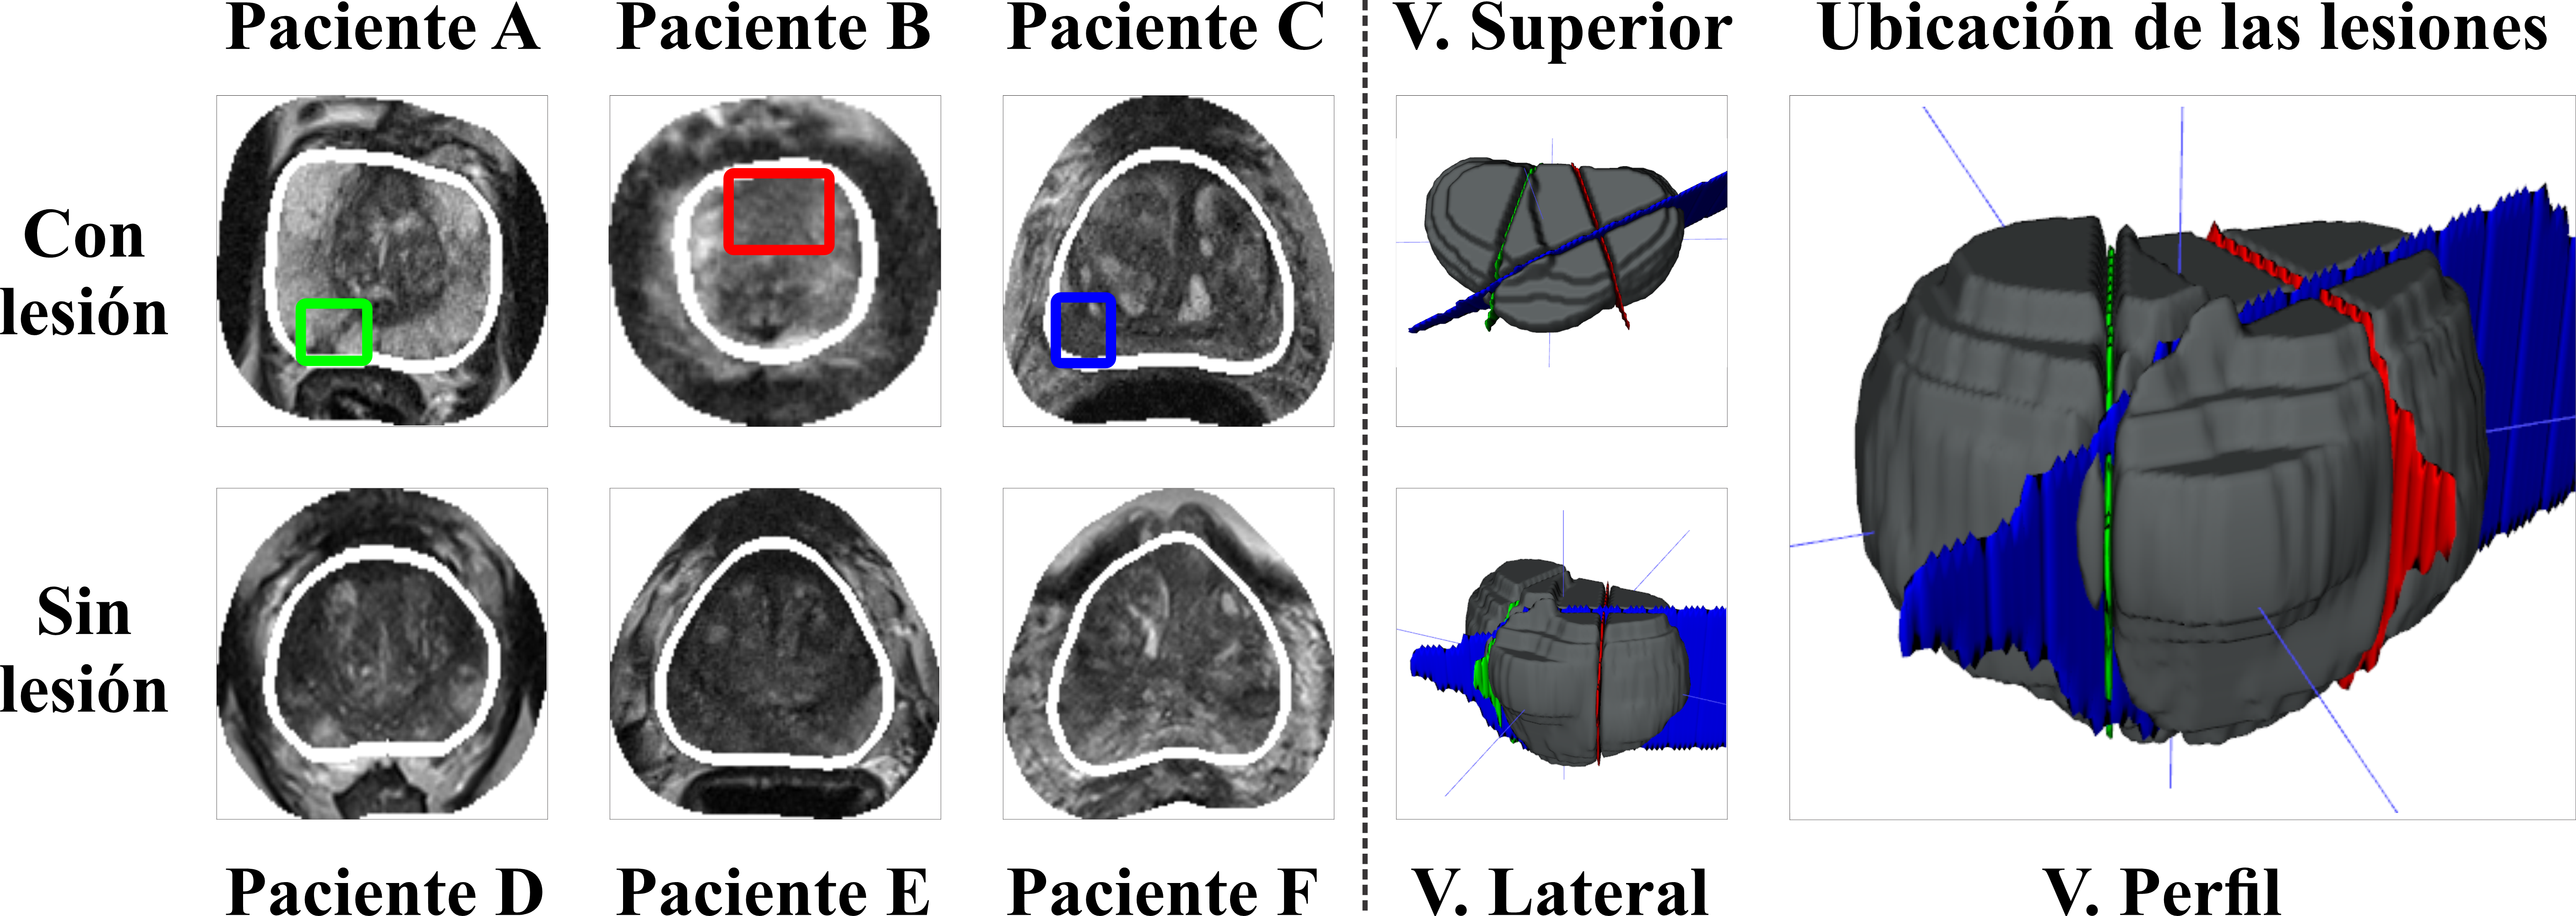
\includegraphics[width=1\textwidth]{imgs/T2WSUMUP.png}
% \caption[Ilustración de lesiones en secuencias T2WI.]{\textbf{Ilustración de lesiones en secuencias T2W.} Imagen construida con el uso de datos bp-MRI de próstata de centros médicos de los Países Bajos \myfootcite{PICAI_BIAS}, y  procesados con el software ITK-SNAP \myfootcite{ITKSNAP}.}
% \label{fig:axT2W}
% \end{figure}

\begin{figure}[h!]
\centering
\caption{Ilustración de lesiones en secuencias T2W.}
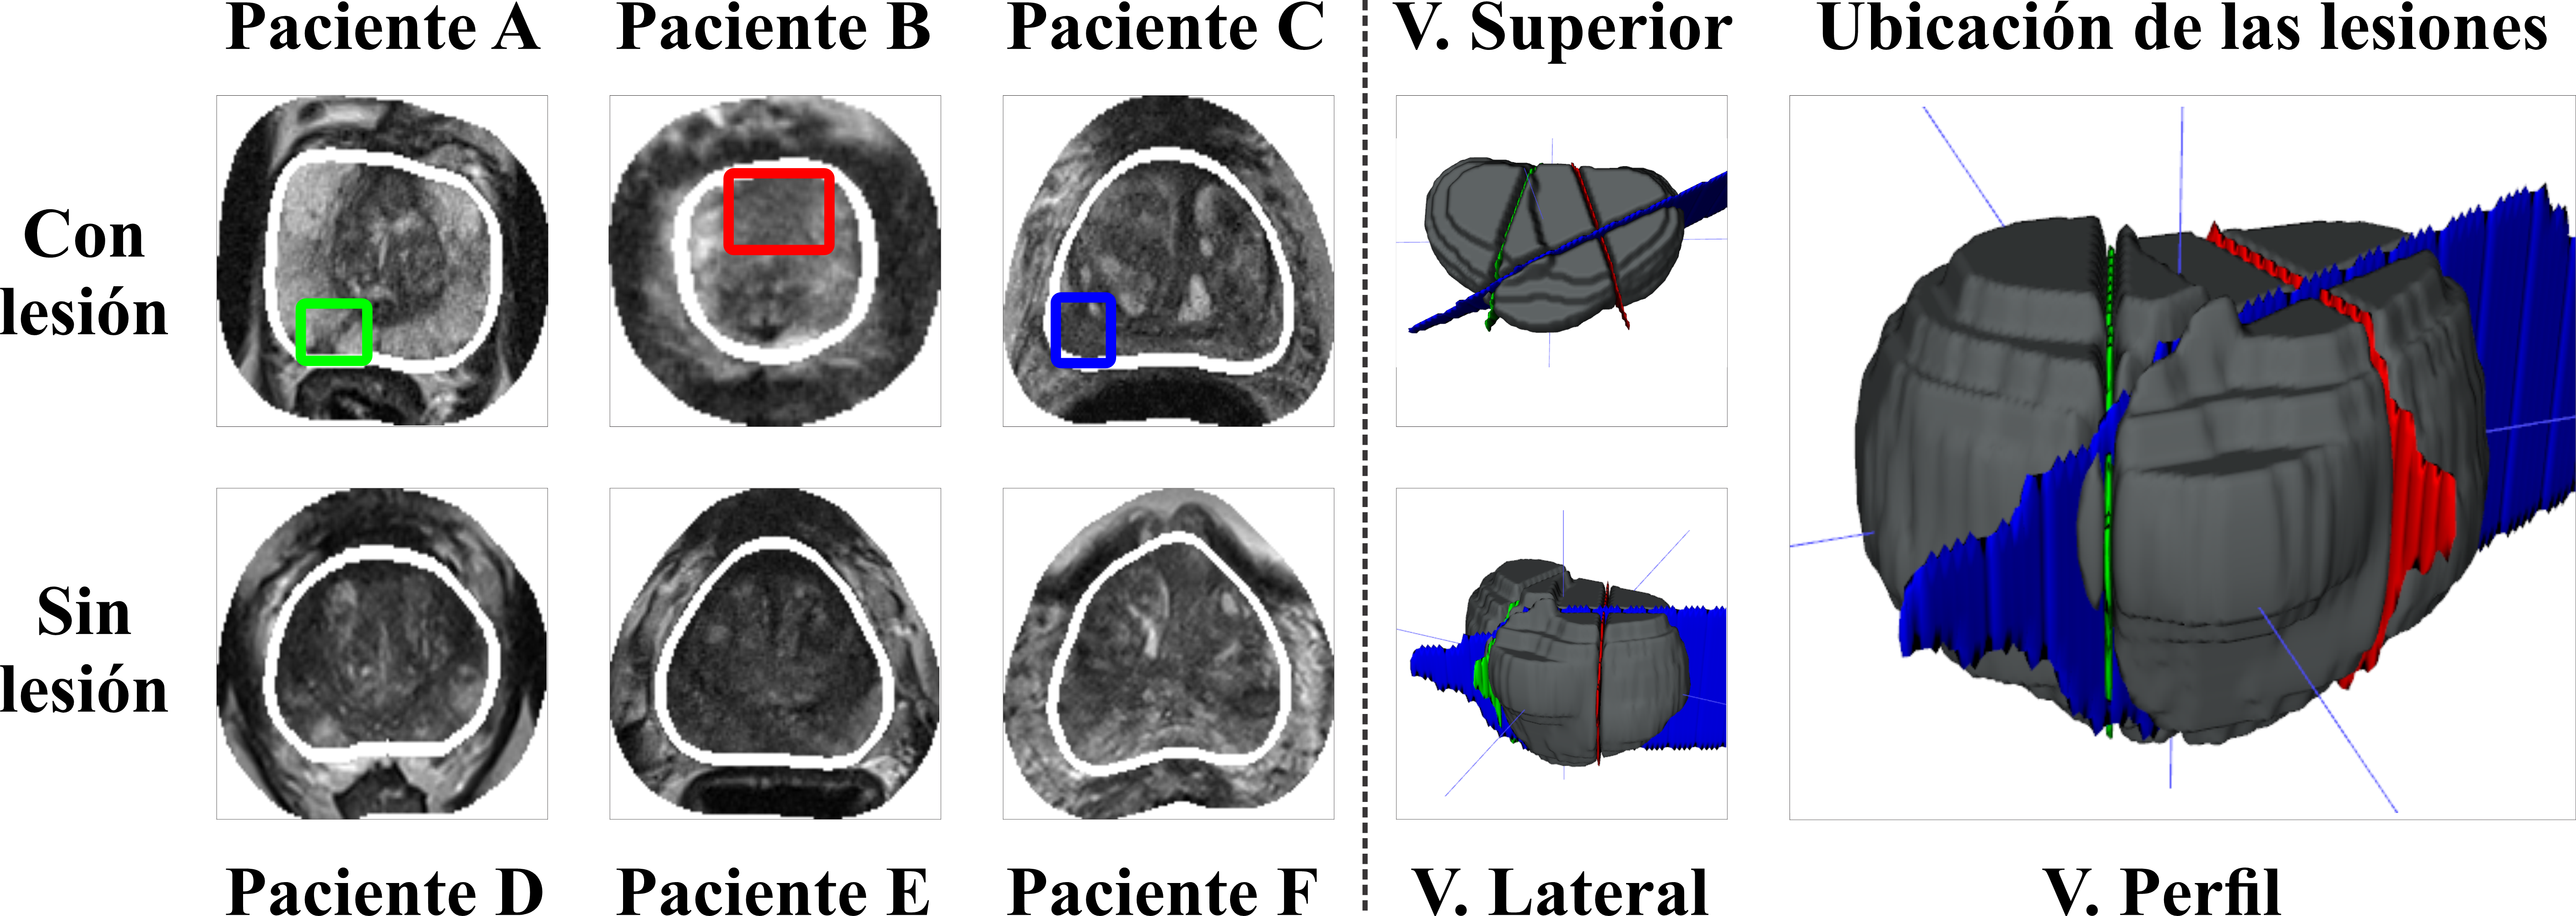
\includegraphics[width=1\textwidth]{imgs/T2WSUMUP.png}
\label{fig:axT2W}
\end{figure}

\begin{figure}[h!]
\noindent \textbf{Nota:} Figura construida con el uso de datos bp-MRI de próstata de centros médicos de los Países Bajos \myfootcite{PICAI_BIAS}, y  procesadas con el software ITK-SNAP \myfootcite{ITKSNAP}.
\end{figure}



\newpage
\subsection{Secuencia de imagen ponderada en difusión (DWI) y mapas ADC. }La secuencia DWI constituye un tipo de imagen que se fundamenta en la movilidad espontánea de las moléculas de agua, conocida como movimiento Browniano \myfootcite{maurer2017diffusion}. Esta secuencia resulta valiosa para obtener información acerca del entorno y los tejidos, debido a que está estrechamente relacionada con las interacciones funcionales del espacio intra y extracelular \myfootcite{Koh2007,Caglic2018}. Característico de esta, es el valor b (b-value), configurable en la adquisición de la secuencia, y connota tiempos y fuerzas de los gradientes que se aplicarán para obtenerla. Convencionalmente, se obtienen secuencias DWI, con diferentes b-value, y es a partir de ellas que se puede llevar a cabo una cuantificación para detectar posibles anormalidades en los tejidos mediante los mapas de Coeficiente de Difusión Aparente (ADC) \myfootcite{lahoti2018role}. Un ADC bajo, que denota un flujo exiguo de agua o difusión reducida, estaría relacionado con tumores o progresiones cancerígenas, que en su mayoría emergen de la producción de biomasa, generando un aumento en la densidad celular y limitando el espacio inter y extracelular disponible. Por el contrario, un flujo desproporcionado podría indicar una degradación celular severa o tejido necrótico \myfootcite{Syer2017,maurer2017diffusion,jacobs2008diffusion}. En la 
%siguientesfiguras (\ref{fig:axDWI}, \ref{fig:axADC}) 
Figura~\ref{fig:axDWI} y Figura~\ref{fig:axADC}
se ilustran cortes de estas secuencias, para diferentes pacientes, además se ilustran casos de glándulas prostáticas con y sin lesión relacionada con el cáncer de próstata. En el panel derecho se muestra una representación volumétrica de la glándula y de los cortes donde se encuentran localizadas las lesiones. 



\begin{figure}[h!]
\centering
\caption{Ilustración de lesiones en secuencias DWI.}
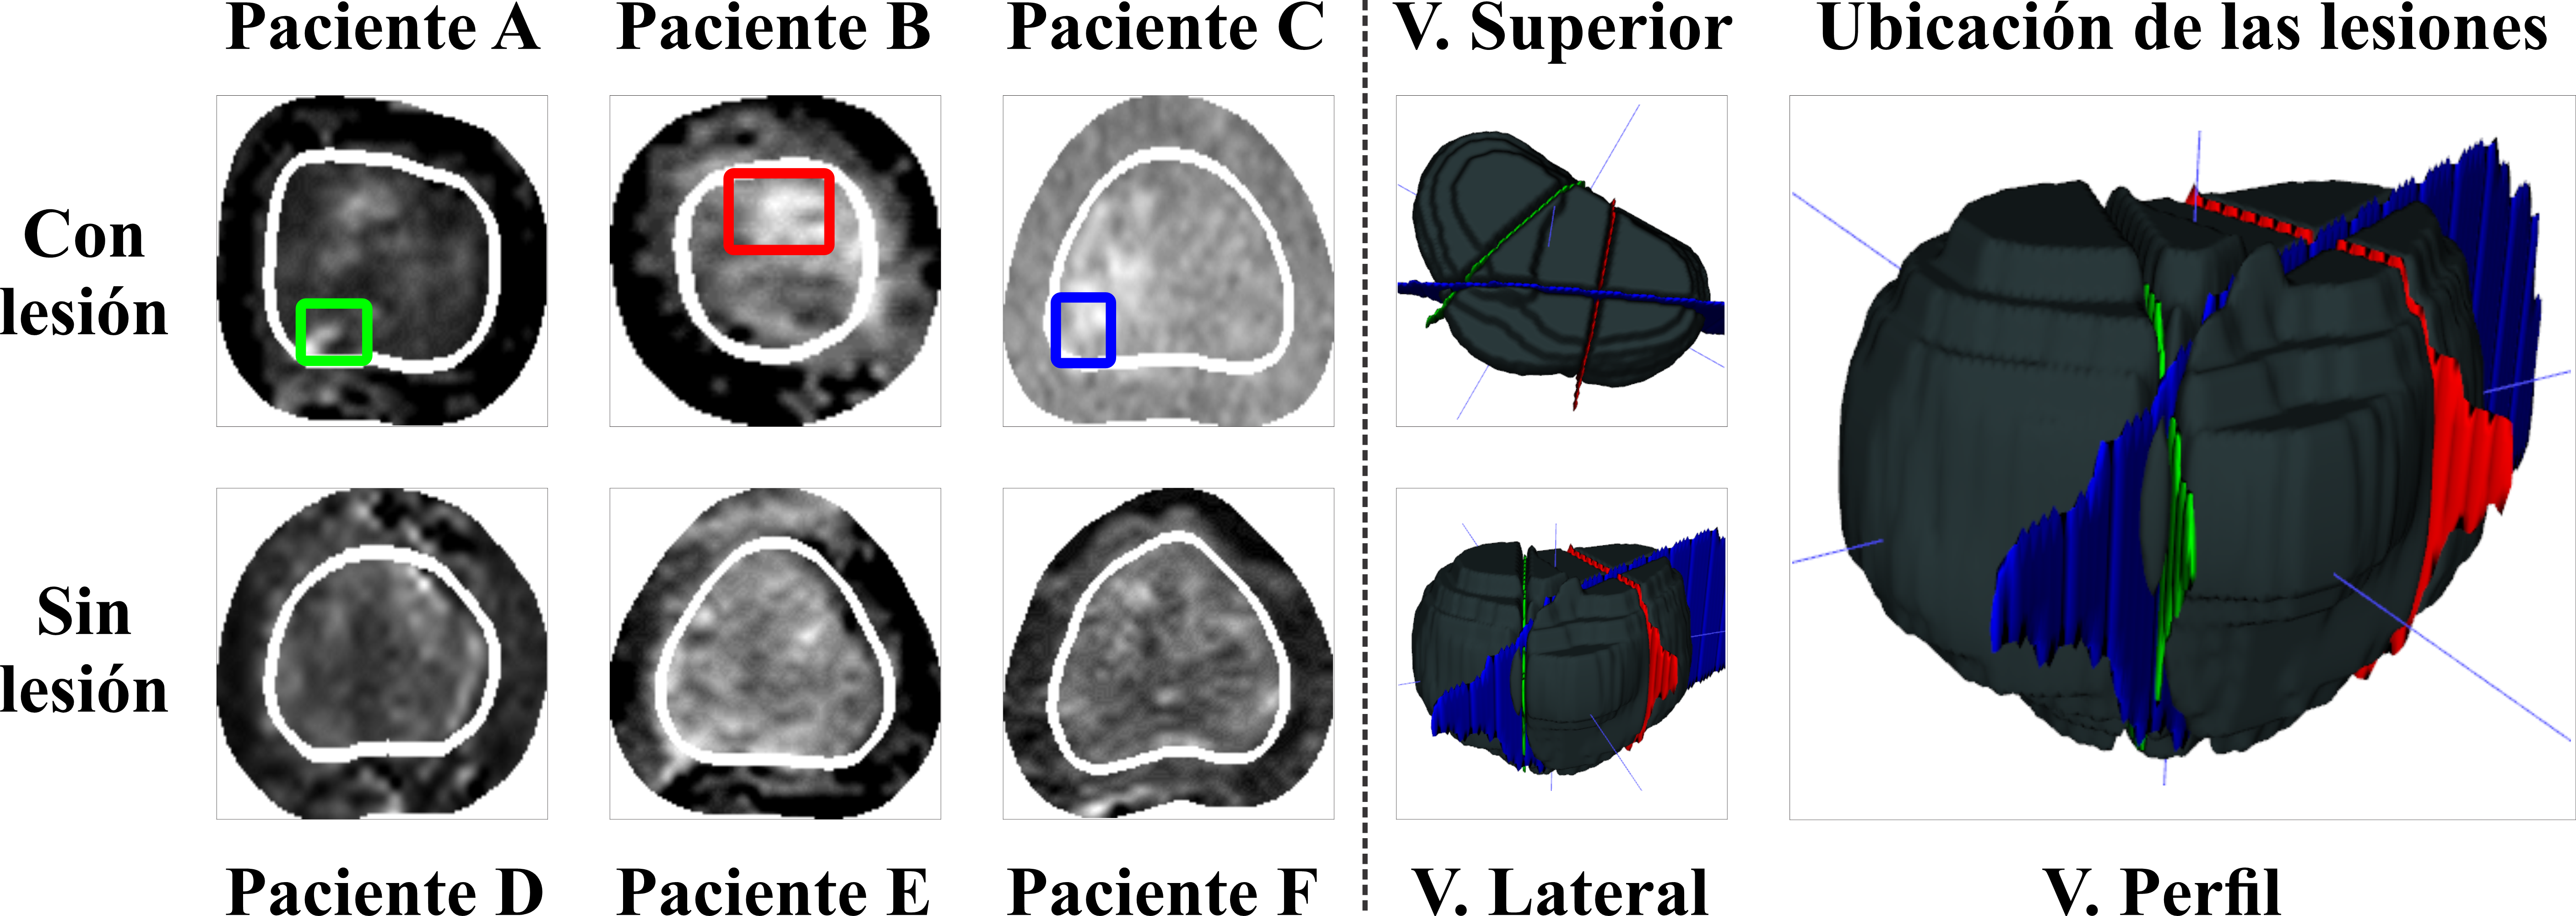
\includegraphics[width=1\textwidth]{imgs/DWISUMUP.png}
\label{fig:axDWI}
\end{figure}

\begin{figure}[h!]
\noindent \textbf{Nota:} Figura construida con el uso de datos bp-MRI de próstata de centros médicos de los Países Bajos \myfootcite{PICAI_BIAS}, y  procesadas con el software ITK-SNAP \myfootcite{ITKSNAP}.
\end{figure}



\begin{figure}[h!]
\centering
\caption{Ilustración de lesiones en secuencias ADC.}
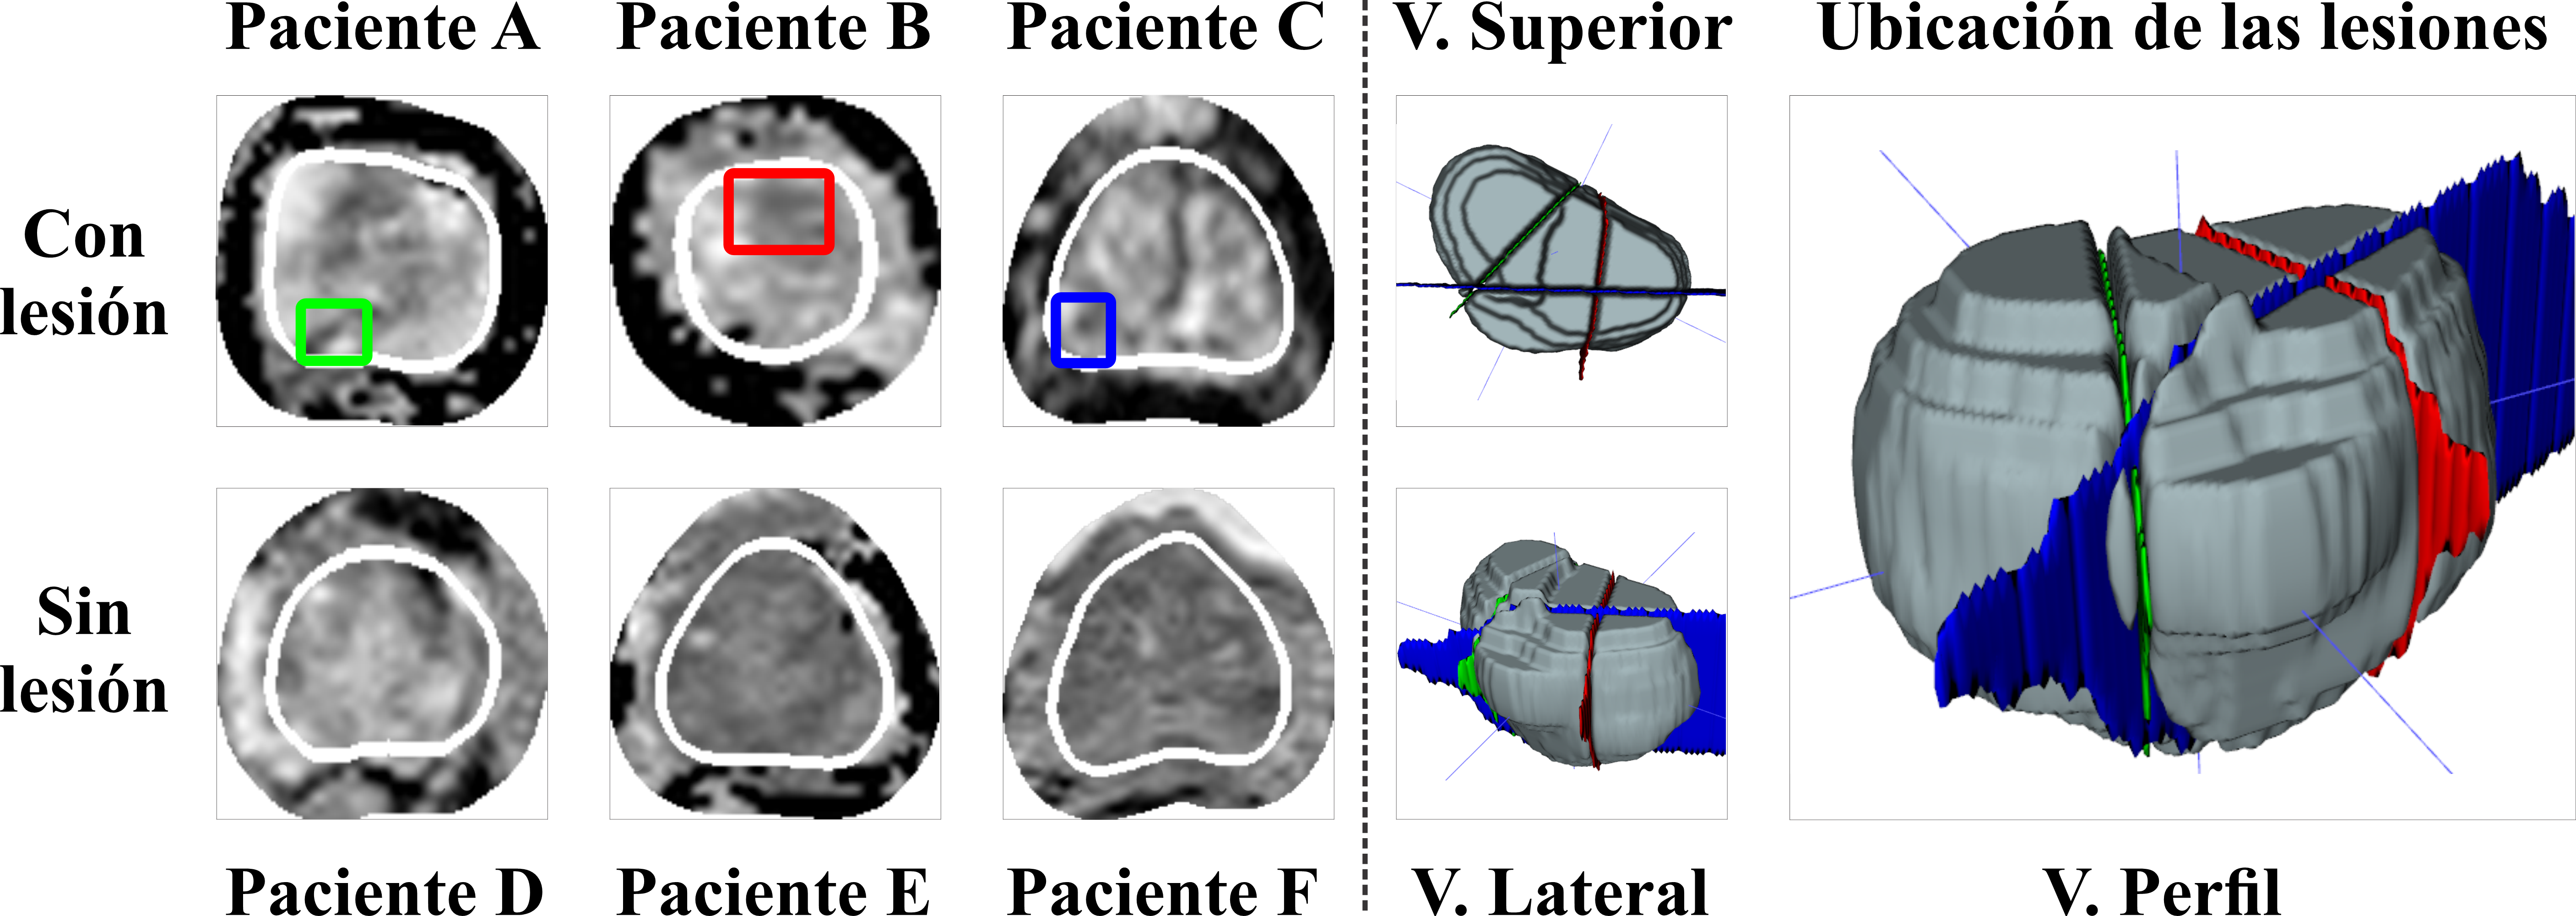
\includegraphics[width=1\textwidth]{imgs/ADCSUMUP.png}
\label{fig:axADC}
\end{figure}

\begin{figure}[h!]
\noindent \textbf{Nota:} Figura construida con el uso de datos bp-MRI de próstata de centros médicos de los Países Bajos \myfootcite{PICAI_BIAS}, y  procesadas con el software ITK-SNAP \myfootcite{ITKSNAP}.
\end{figure}






\newpage
\section{ESTRATEGIAS COMPUTACIONALES DE LOCALIZACIÓN} \label{sec:comp_localiza}
En esta sección se realiza un breve compendio sobre herramientas que se han propuesto para la tarea de localización. 
Para esto, se pueden identificar tres categorías principales en las que se agrupan estos métodos: sistemas de ventana deslizante, sistemas de búsqueda selectiva y sistemas basados en una única observación.

\subsection{Sistemas de ventana deslizante. }% - Haar [25], SIFT [23], HOG [4]
Los sistemas de ventana deslizante son técnicas que fueron ampliamente utilizadas para el procesamiento de imágenes y la detección de objetos de interés. Estos sistemas se basan en la aplicación de un escaneo a diferentes regiones de la imagen, obtenidas mediante el desplazamiento de una ventana o cuadrícula de tamaño fijo a lo largo de la misma. Para mejorar el rendimiento en detección, se ha propuesto extraer características relevantes de las regiones de la ventana, por ejemplo, a través de una muestra local que estime información relevante, y a su vez, escanee cambios en la imagen \myfootcite{DeCroon200797}. Algunos ejemplos de sistemas de ventana deslizante son los basados en las características de Haar wavelet (Haar), Scale-Invariant Feature Transform (SIFT) o Histogram of Oriented Gradients (HOG).\par
Los sistemas basados en Haar propenden por hallar diferencias basadas en la variación de intensidad entre regiones adyacentes de la imagen, con la finalidad de establecer representaciones estructurales, que serán posteriormente procesados por clasificadores como máquinas de soporte vectorial (SVM, por sus siglas en inglés) \myfootcite{Papageorgiou2000}. En la literatura, este método es combinado con un algoritmo de aprendizaje llamado AdaBoost para mejorar la capacidad de discriminación entre objetos y fondos. Esta estrategia es conocida por su eficiencia y mejora en la precisión, por ejemplo, para tareas de detección de objetos \myfootcite{V.Jones}. Por otra parte, el sistema SIFT busca extraer características que sean distintivas e invariantes de las imágenes, aún cuando le son aplicadas transformaciones o quizás distorsiones, como escalamientos, rotaciones, ruido, iluminación y demás cambios de apariencia, esto mediante la asignación de un descriptor basado en el gradiente local. El método es ampliamente utilizado para el reconocimiento de objetos y ha demostrado ser efectivo incluso en escenarios con problemas de oclusión, logrando además, un rendimiento casi de tiempo real \myfootcite{Lowe2004}. Finalmente, los sistemas basados en HOG utilizan distribuciones probabilísticas de los gradientes locales en diferentes regiones de la imagen para de esta forma capturar de mejor manera características invariantes. Posteriormente, estas distribuciones alcanzadas son utilizadas para entrenar un clasificador lineal como SVM. \myfootcite{Dalal-Hog}. Algunas de estas metodologías han sido utilizadas para recalar en la localización y detección de lesiones prostáticas en MRI \myfootcite{Qian2016,Lay2017}.

% A pesar de su utilidad, los sistemas de ventana deslizante presentaron algunos desafíos. Por ejemplo, requieren evaluar muchas regiones candidatas, lo que puede ser computacionalmente costoso, además pueden producir múltiples detecciones del mismo objeto, lo que requiere mecanismos, no siempre efectivos para tratar redundancias, así mismo, pueden tener dificultades para adaptarse a variaciones en la forma, pose u oclusión del objeto, lo que afecta su robustez, eficacia o representatividad del aprendizaje.




\subsection{Sistemas de búsqueda selectiva. }Con el antecedente de las redes convolucionales (CNN), los sistemas de búsqueda selectiva afloran como una propuesta para generar conjuntos de regiones candidatas, que puedan contener objetos, para una ulterior clasificación. Por ejemplo, el algoritmo \textit{Regions with CNN features} (R-CNN) para la detección de objetos, combina la postulación de regiones con las características extraídas por una red neuronal convolucional (CNN).
% Este algoritmo demostró significativas mejoras en precisión, su funcionamiento se estructura en tres etapas.
Propiamente, este algoritmo genera propuestas de regiones por imagen, luego extrae un vector de características que se proyecta a un clasificador \myfootcite{Girshick2014}. La R-CNN cuenta con diferentes actualizaciones y mejoras entre las que se enmarca la Fast R-CNN, la Faster R-CNN y la Mask R-CNN \myfootcite{RCNNfamily}. \par La primera, Fast R-CNN, postula una red que se encarga del proceso de proponer regiones, haciéndolo de manera más eficiente. Esta red también se reconoce por la introducción del concepto Region of Interest (RoI) Pooling, empleado para proyectar las regiones candidatas sobre los mapas de características de la CNN \myfootcite{GiFast}. En consideración, la Faster R-CNN basa su detección en la Fast R-CNN, agregando una red de propuestas de regiones (RPN, region proposal network), que dispensa del algoritmo de búsqueda selectiva. Además, realiza la tarea directamente desde el mapa de características de la CNN, acelera el proceso de detección, se destaca que comparten características convolucionales con la red de detección \myfootcite{RenFaster}. Por otra parte, fue introducida la Mask R-CNN, que adiciona un proceso de segmentación semántica, donde se añade una rama paralela que genera una máscara binaria para cada región candidata. De esta forma, Mask R-CNN puede producir no solo la clase y la caja delimitadora del objeto, sino también una delineación del contorno del objeto  \myfootcite{heMask}. Estas arquitecturas en relación al cáncer de próstata han sido integradas en etapas de preprocesamiento \myfootcite{Soni2022,Dai2021,Liu2019}.


\subsection{Sistemas basados en una única observación. }Los sistemas de detección de objetos en imágenes basados en una única observación son una aplicación innovadora que abrió nuevas perspectivas en el campo de visión por computador. Algunos de los sistemas que operan bajo este concepto incluyen You Only Look Once (YOLO) \myfootcite{RedYolo}, Single Shot MultiBox Detector (SSD) \myfootcite{LiuSSD}, RetinaNet \myfootcite{LinRetin}, SpineNet \myfootcite{DuSpine} y DEtection TRansformer (DETR) \myfootcite{CarionDetr}. \par

A diferencia de los algoritmos de sistema de búsqueda selectiva, estos algoritmos realizan la detección de objetos en una sola pasada a través de la red neuronal y utilizan diferentes estrategias para mejorar la precisión y el equilibrio entre las clases de objetos. Por ejemplo, la estrategia YOLO es una técnica de detección de objetos en tiempo real que propone dividir la imagen en una cuadrícula de celdas, sobre las cuales se ejecutarán tareas de detección. Para esto, en cada celda son propuestos unos cuadro delimitadores, a los cuales, durante el entrenamiento se les asigna puntuaciones, en referencia a la confianza y precisión por la existencia de un objeto de cierta clase en dicho cuadro delimitador. La red ajusta también la ubicación y el tamaño de los cuadros delimitadores, maximizando su precisión de forma que se seleccione el cuadro más confiable. Específicamente, la red YOLO involucra una función de pérdida que tiene en cuenta varios factores: la precisión de la localización del cuadro delimitador, la confianza de la detección y la precisión de la clasificación de objetos. Su uso se ha extendio a tareas como la vigilancia, la conducción autónoma, incluso el reconocimiento de imágenes \myfootcite{RedYolo}. Por su parte, Single Shot MultiBox Detector (SSD) es una propuesta para detección en tiempo real, que a diferencia de la YOLO, busca simplificar y ser mas eficiente en el proceso de selección de los cuadros delimitadores. Esto lo logra mediante un enfoque multi-escala, el cual mejora la detección de objetos de diferentes tamaños al hacer el análisis de cajas delimitadoras sobre características de diferente resolución. De manera similar a la YOLO, la red genera puntuaciones para la presencia de cada categoría de objeto en cada caja delimitadora. Además, se combinan las predicciones de los múltiples mapas de características, incluyendo así una detección mas robusta que trate con diferentes tamaños de objeto \myfootcite{LiuSSD}. Sin embargo, esta robustez de las características alcanzadas en esta red, dependen de los cuadro delimitadores definidos desde un inicio. A partir de esto, surge RetinaNet, una red para detección de objetos que se compone de una CNN  de tipo ResNet, y cuya principal contribución se centra en la introducción de una Feature Pyramid Network (FPN). FPN toma características profundas y crea una piramide de caracteristicas a diferente grado de resolución. Seguidamente, se utilizan dos subredes: una de clasificación para los niveles de la FPN, regida por una pérdida focal que soporta el problema de desbalance de clases en imágenes con mucho fondo, esto asignando un mayor peso a las cajas delimitadoras que contienen objetos difíciles de detectar o poco frecuentes; y una segunda red dedicada a la predicción a través de regresión, de los centros y áreas de las cajas delimitadoras. Los experimentos muestran que la RetinaNet, con la pérdida focal propuesta, supera a los detectores que la anteceden \myfootcite{LinRetin}. 
En vía de crear una mejor fusión de características multi-escala, el equipo de Google propuso la SpineNet. Esta propuesta identifica como un problema para la tarea de localización y detección, la captura de características a través de una reducción espacial, como lo hace el método involucrado en la FPN. Por el contrario, introducen un método más eficaz con un backbone dinámico, donde los mapas de características se proyectan a través de conexiones entre diferentes escalas. Para esto, la SpineNet utiliza técnicas de diseño automático de arquitectura (NAS, por sus siglas en ingles \textit{Neural Architecture Search}). Como resultado, demuestran que esta estrategia permite capturar mejor la información espacial y fusionar mejor la información, dos aspectos claves en tareas de detección \myfootcite{DuSpine}. Por último, se han propuesto recientemente redes que involucran mecanismos de atención mediante la introducción de arquitecturas \textit{Transformer} en el codificador extractor de características y generador de las cuadros candidatos. Este tipo de estrategias permiten refinar las predicciones de las clases y las ubicaciones de los cuadros, utilizando incluso varias redes de atención de múltiples cabezas \myfootcite{CarionDetr}. Estos enfoques han sido aproximados para el cáncer de próstata en \myfootcite{Salman2022,Seetharaman2021}.



\section{ANTECEDENTES LOCALIZACIÓN DE LESIONES CS-PCA}\label{sec:localiza_pca}Para el personal médico radiológico el diagnóstico de lesiones csPCA en imagenología MRI es una tarea compleja que requiere una amplia experticia, y aún teniéndola, persiste gran variabilidad de interpretación dependiendo del lector \myfootcite{Twilt2021}. El desarrollo de herramientas diagnósticas basadas en computador (CAD, Computer aided diagnosis), y en especial aquellas apoyadas por inteligencia artificial, resultan entonces fundamentales para soportar la detección de lesiones anormales y su correspondiente diagnóstico \myfootcite{Mata2021,Harmon2019}. Para el caso del soporte a labores urológicas, estas herramientas pueden mejorar la especificidad y la eficiencia del experto radiólogo, en especial cuando existen lesiones en zonas difíciles de interpretar, como sucede en lesiones ubicadas en la zona transicional de la próstata \myfootcite{murphy2013expanding}. A razón de ello, estas herramientas pueden contribuir a la reducción de variabilidad inter-lector \myfootcite{Gaur2018}. En los protocolos clínicos existen acuerdos y protocolos clínicos que establecen la importancia de utilizar los diferentes parámetros MRI, por la significancia que cada una de ellas brinda para la localización y diagnóstico final \myfootcite{Scott2021,maurer2017diffusion,Wu2019}. Es por esto, que las herramientas propuestas deben tener en primer lugar la capacidad de capturar, ubicar y cuantificar patrones radiómicos de importancia, con la finalidad de obtener herramientas óptimas que permitan posteriormente una evaluación final por parte del lector \myfootcite{Algohary2018}. Por consiguiente, se introducirán a continuación herramientas de localización y detección propuestas a la fecha.\par

Una primera aproximación común para esta tarea en imágenes MRI de próstata ha sido el análisis por regiones. En ese sentido, (Qian et al., 2016) propuso un framework que involucraba una interpretación de todas las regiones de la próstata mediante el análisis del contexto en las estructuras de los tejidos \myfootcite{Qian2016}. Por su parte, en \myfootcite{Lay2017}, se incorporó la ponderación de instancias para evitar sesgos con el volúmen de cada lesión, así como el uso de delineaciones manuales de la próstata.  Aunque estos dos métodos obtienen buenos resultados, sus estudios fueron realizados con una limitada cantidad de datos, afectando posiblemente su capacidad de generalización y representación. Además, el enfoque de estos se basa en los primeros sistemas de localización de ventana deslizante y clasificadores como bosques de decisión (DTs) y SVM, no especializados en la extracción de características de la imagen para la tarea de localización. Para esto, posteriormente se postularon redes de extremo a extremo que vinculan dos subredes para las tareas de registro y detección mediante la introducción de CNNs \myfootcite{Le2017,Wang2018}. A pesar de alcanzar buenos resultados en cuanto a sensibilidad y especificidad, el primero enuncia valores bajos de especificidad, que podría inducir errores, hasta someter pacientes a tratamientos innecesarios, mientras el segundo muestra una baja sensibilidad, que podría desestimar pacientes con lesiones significativas que requieran atención y tratamiento. A partir de esto, otros trabajos propusieron enfoques similares, destinando redes CNN extremo a extremo en sus desarrollos \myfootcite{Ishioka2018,Sumathipala2018,Cao2019}. Así mismo, se han propuesto trabajos que buscan alcanzar una mejor localización utilizando información mapeada desde imágenes histopatológicas \myfootcite{Dai2021,Seetharaman2021}, inclusive, autores como (Salman et al., 2022) han propuesto el uso de la herramienta YOLO, para maniobrar la localización del cáncer de próstata \myfootcite{Salman2022}. Sin embargo, estos enfoques involucran el registro de imágenes MRI e histopatológicas, lo cual puede carecer de una buena congruencia y verse afectado por una mala correspondencia entre las imágenes. Por otra parte, la evolución de diferentes estrategias en CNNs ha permitido que emerjan nuevos métodos, por ejemplo, involucrando módulos residuales, utilizando transfer learning, e incluso, incluyendo mecanismos de atención para segmentación \myfootcite{Xu2019,Abbasi2020,Mehralivand2020}. 
% , mas, sus desarrollos se basaron también en datos monocentro. Por otra parte, también se han involucrado 
No obstante, este último enfoque no alcanza resultados satisfactorios, sugieren que es necesario un conjunto de datos óptimos con buen procesamiento, e incluso que incluya estudios de diferentes centros para capturar mejor la alta variabilidad que concierne a las lesiones prostáticas en MRI \myfootcite{Mehralivand2020}. Además, explicitan que tareas de clasificación de lesiones no parecerían muy adecuadas, pues es ciertamente subjetiva y dificulta la tarea de segmentar la lesión.
Enfoques similares de segmentación, como los modelos Panópticos \myfootcite{Xu2019}, donde metodología semántica y segmentación de instacias fueron involucradas, arrojaron mejoras en el rendimiento de detección. 
De la misma manera, existen abordajes 3D, donde buscan enfocarse en características relevantes en múltiples resoluciones a través de mecanismos de atención y CNNS 3D \myfootcite{Saha2021}, así mismo, involucran información de dominio clínico para sus desarrollos. También, los autores resaltan la importancia de diversificar en herramientas CAD que resulten menos dependientes a los conjuntos de datos. Recientemente, se han decantado por aproximarse a soluciones retomando métodos de KNN, donde se refieren a  matrices de concurrencia, o reducción de ruidos por transformaciones, hasta clasificadores tradicionales \myfootcite{Anand2023}. Sin embargo, es claro que estructuras especializadas en imágenes han mostrado ser más eficientes. Otras soluciones involucran esquemas adversarios-generativos (Gans, por sus siglas en Inglés) \myfootcite{Patsanis2023}. No obstante, su propuesta desestiman las características radiómicas variopintas al no involucrar secuencias anatómicas y funcionales MRI, donde en la práctica médica, y además, en bpMRI, ninguna es sustitutoria.\par De esta manera, es evidente que, aunque los desarrollos relacionados con la detección de lesiones CsPCA son importantes, su enfoque propositivo de frameworks propios y esfuerzos en tareas de clasificación, podrían llevar a un descuido o desaprovechamiento de las herramientas de localización que conforman el estado del arte, las cuales han sido probadas y validadas por la comunidad académica y han demostrado ser efectivas y confiables.\pagebreak
